{\centering \nonumsubsection{A \hspace{1em} 组}}
\begin{xiaotis}
\begin{enhancedline}

\xiaoti{$AB$、$BC$、$CD$ 是不在同一平面内的线段。求证:经过它们中点的平面和 $AC$ 平行,也和 $BD$ 平行。}

\xiaoti{如图,$AB$ 是圆 $O$ 的直径,$PA$ 垂直于圆 $O$ 所在的平面,$C$ 是圆周上的任意点。
    求证:$\triangle PAC$ 所在的平面垂直于 $\triangle PBC$ 所在的平面。
}

\begin{figure}[htbp]
    \centering
    \begin{minipage}[b]{7cm}
        \centering
        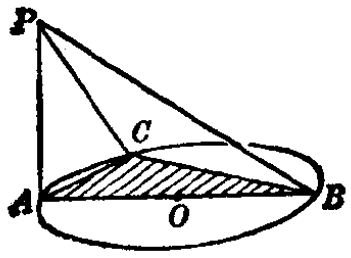
\includegraphics[width=4cm]{../pic/ltjh-zongfuxi-02.png}
        \caption*{(第 2 题)}
    \end{minipage}
    \qquad
    \begin{minipage}[b]{7cm}
        \centering
        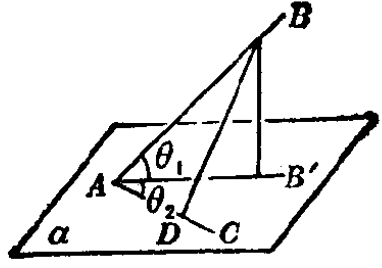
\includegraphics[width=4cm]{../pic/ltjh-zongfuxi-03.png}
        \caption*{(第 3 题)}
    \end{minipage}
\end{figure}

\xiaoti{如图,$AB$ 和平面 $\alpha$ 所成的角是 $\theta_1$,$AC$ 在平面 $\alpha$ 内,
    $AC$ 和 $AB$ 的射影 $AB'$ 成角 $\theta_2$,设 $\angle BAC = \theta$。 求证:
    $$ \cos\theta_1 \cdot \cos\theta_2 = \cos\theta \juhao $$
}

\xiaoti{在 $60^\circ$ 的二面角 $\alpha{-}AB{-}\beta$ 中, $AC \subset \alpha$, $BD \subset \beta$,
    且 $AC \perp AB$,$BD \perp AB$。已知 $AB = AC = BD = a$,求 $CD$ 的长。
}

\xiaoti{将正方体截去一个角。 求证:截面是锐角三角形。}

\xiaoti{已知圆锥底面半径是 $r$,母线长是 $2r$,用平行于底面的平面把这个圆锥表面截成相等两部分。
    求截下的圆锥的母线长。
}

\xiaoti{要使电视卫星的电波,能直射到地球表面积的 $\exdfrac{1}{3}$,卫星要发射到多高?}



\xiaoti{三棱锥 $S{-}ABC$ 中,侧棱 $SA$、$SB$、$SC$ 的长分别是 $a$、$b$、$c$,
    又 $\angle ASB = 60^\circ$, $\angle ASC = \angle BSC = 90^\circ$,
    求这个棱锥的体积。
}

\xiaoti{圆柱的底面半径是 10 cm,高是 15 cm,平行于轴的截面在底面上截得的弦等于底面半径。
    求圆柱被截去部分的体积。
}

\xiaoti{圆台的两底面半径分别是 $a$ 和 $b$($a > b$)。求这个圆台的体积与截得它的圆锥的体积的比。}

\xiaoti{面积为 $2512\;\pflm$ 的铝板,经冲压制成圆柱形铝桶,如果铝桶的面积和铝板面积相等,
    高是 $10\;\limi$。 求这种铝桶的容积。
}

\xiaoti{长江大桥的钢梁结构是用铆钉铆合的(如图,单位:mm)。铆钉头是球缺形,钉身是圆柱形,
    铆钉插入两块钢板铆合后,两侧钉头大小相等。 已知每块钢板厚 12 mm,求钉身长度。
}

\begin{figure}[htbp]
    \centering
    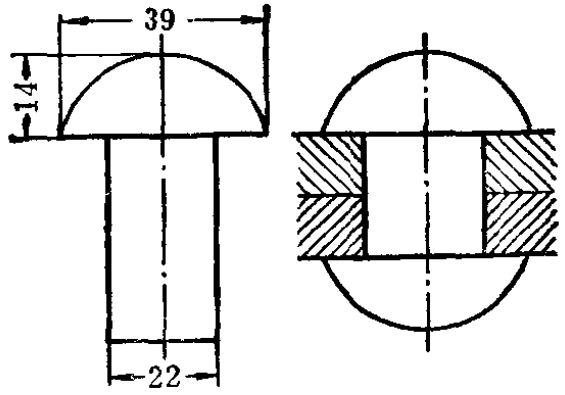
\includegraphics[width=6cm]{../pic/ltjh-zongfuxi-12.png}
    \caption*{(第 12 题)}
\end{figure}


\xiaoti{分别以直角三角形的斜边、两直角边所在直线为轴,旋转这个直角三角形所得的三个旋转体的体积为 $V$、$V_1$、$V_2$。求证:
    $$ \dfrac{1}{V^2} = \dfrac{1}{V_1^2} + \dfrac{1}{V_2^2} \juhao $$
}

\xiaoti{正方体、等边圆柱(即底面直径与母线相等)、球的体积相等时,哪一个全面积最小?}


\begin{withstar}

\xiaoti{从平面外一点向平面引两条斜线,其中一条与平面成 $70^\circ$ 角,
    另一条与平面成 $15^\circ$ 角。求这两条斜线组成的最大角、最小角各为多少度。
}

\end{withstar}

\end{enhancedline}
\end{xiaotis}
